% This is a shared SUNDIALS TEX file with description of
% the SUNDIALS organization
%
The family of solvers referred to as {\sundials} consists of the solvers
{\cvode} and {\arkode} (for ODE systems), {\kinsol} (for nonlinear algebraic
systems), and {\ida} (for differential-algebraic systems).  In addition,
{\sundials} also includes variants of {\cvode} and {\ida} with sensitivity analysis 
capabilities (using either forward or adjoint methods), called {\cvodes} and
{\idas}, respectively.

The various solvers of this family share many subordinate modules.
For this reason, it is organized as a family, with a directory
structure that exploits that sharing (see Figs. \ref{f:sunorg1} and \ref{f:sunorg2}).
%%
%%
\begin{figure}
{\centerline{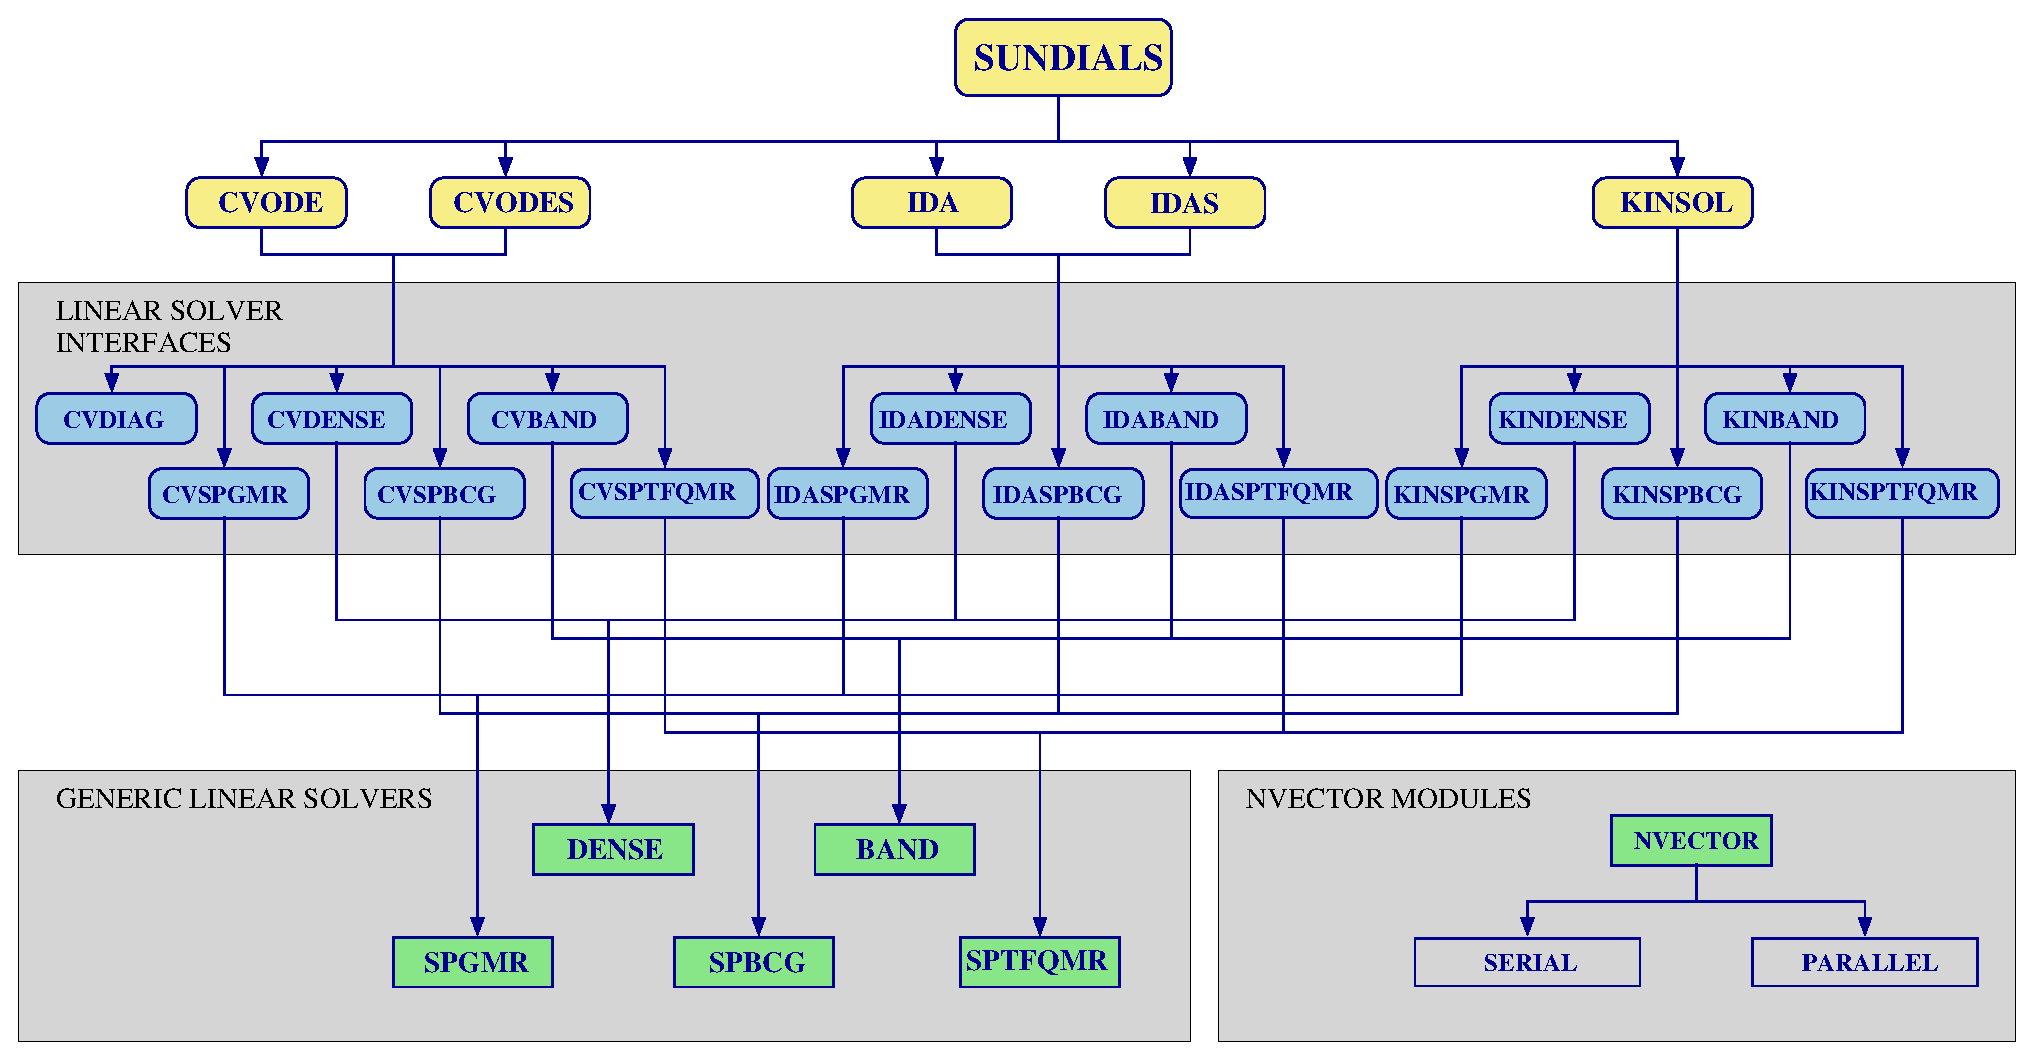
\includegraphics[width=\textwidth]{sunorg1}}}
\caption {High-level diagram of the {\sundials} suite}\label{f:sunorg1}
\end{figure}
%%
%%
\begin{figure}
\subfigure[Directory structure of the {\sundials} source tree]
{\centerline{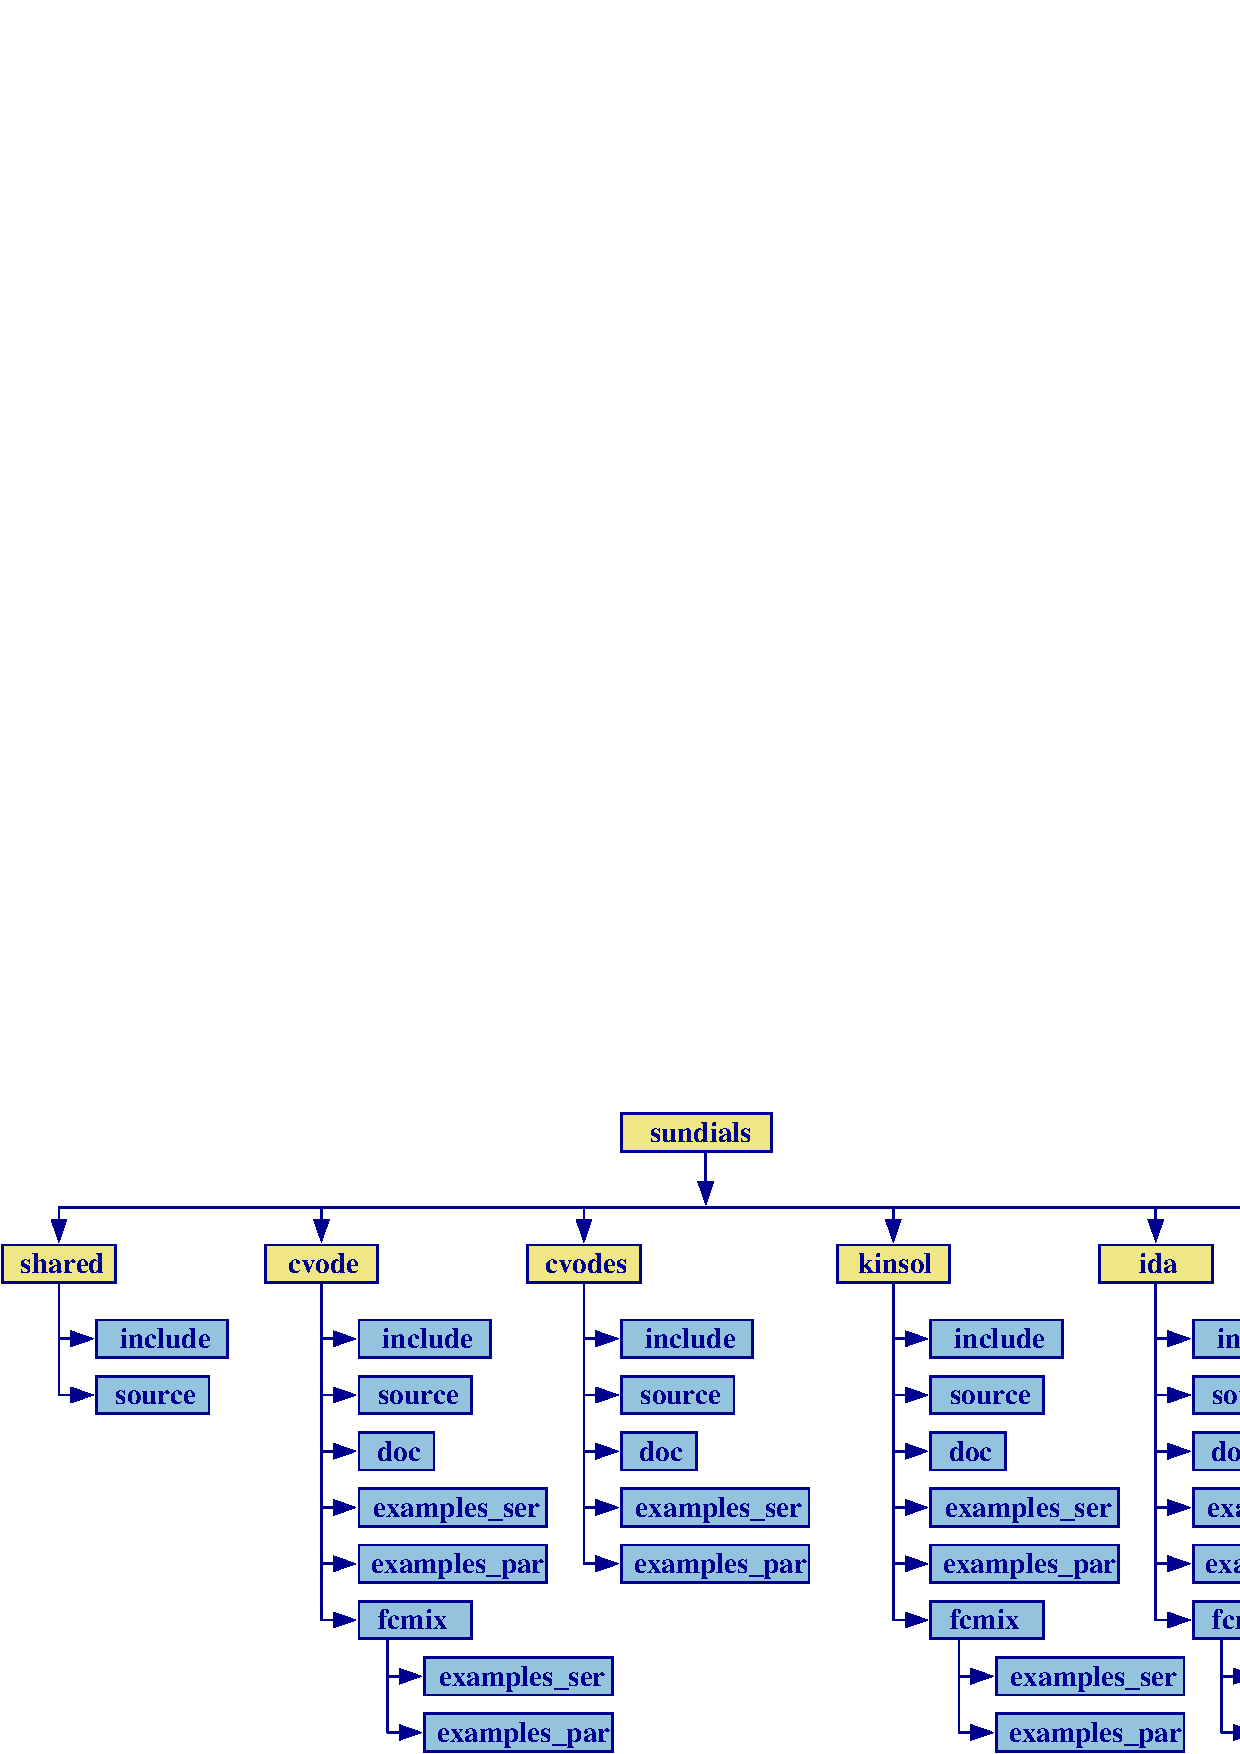
\includegraphics[width=\textwidth]{sunorg2}}}
\subfigure[Directory structure of the {\sundials} examples]
{\centerline{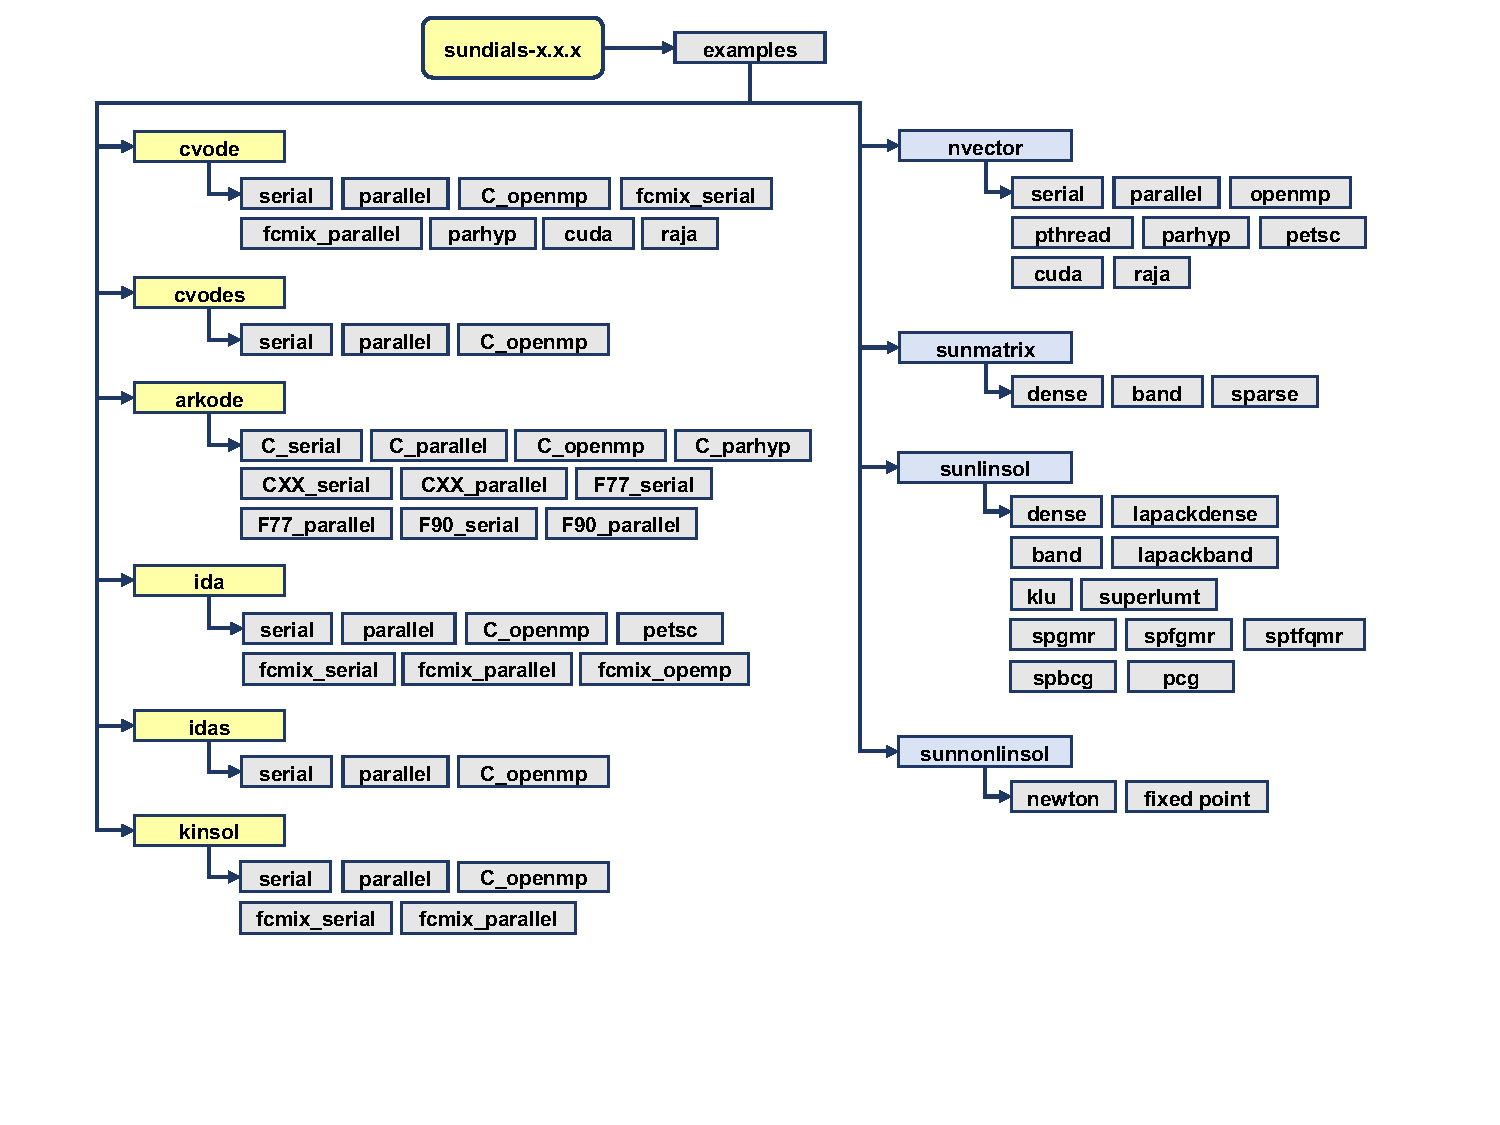
\includegraphics[width=\textwidth]{sunorg3}}}
\caption {Organization of the {\sundials} suite}\label{f:sunorg2}
\end{figure}
%%
%%
The following is a list of the solver packages presently available, and
the basic functionality of each:
\begin{itemize}

\item {\cvode},  
  a solver for stiff and nonstiff ODE systems $dy/dt = f(t,y)$ based
  on Adams and BDF methods;

\item {\cvodes},
  a solver for stiff and nonstiff ODE systems with sensitivity analysis capabilities;

\item {\arkode},
  a solver for ODE systems $M dy/dt = f_E(t,y) + f_I(t,y)$ based on
  additive Runge-Kutta methods; 

\item {\ida},
  a solver for differential-algebraic systems $F(t,y,\dot{y}) = 0$ based on BDF methods;

\item {\idas},
  a solver for differential-algebraic systems
  with sensitivity analysis capabilities;

\item {\kinsol}, 
  a solver for nonlinear algebraic systems $F(u) = 0$.

\end{itemize}
